\documentclass[11pt]{article}

%Both greek and english language support
\usepackage[greek,english]{babel}
\usepackage{alphabeta}
\usepackage[utf8]{inputenc}

% For \includegraphics
\usepackage{graphicx}   
\usepackage[space]{grffile}

% Maths extra
\usepackage{amsmath}
\usepackage{amssymb}

\usepackage{float}

%Todo notes
% \usepackage[colorinlistoftodos]{todonotes}

% Page margins 
\usepackage{geometry}
 \geometry{
 a4paper,
 total={170mm,257mm},
 left=20mm,
 top=20mm,
 }

%Negative exponential
\DeclareUnicodeCharacter{2212}{-}   

\begin{document}
%--------------------------------------------------------------------------------------------
% Title Page
\begin{titlepage}
    \center
    %----------------------------------------------------------------------------------------
    %	HEADING SECTIONS
    \textsc{\LARGE Technical University of Crete}\\[2cm] 
    \Large Ψηφιακή Επεξεργασία Σήματος\\
    \emph{ΤΗΛ302}\\[1cm] 
    
    \rule{\linewidth}{0.5mm} \\[0.5cm]
        { \huge \bfseries Εργαστήριο 2}\\[0.5cm]
    \rule{\linewidth}{0.5mm} \\[2.5cm]
    
    \begin{minipage}{0.4\textwidth}
        \begin{flushleft} \large
            \emph{Authors:}\\
                Ισίδωρος Πατεράκης AM: 2017030091
                Μαρίνου Ιωάννα AM: 2016030143
                Σπυριδάκης Χρήστος AM: 2014030022
        \end{flushleft}
    \end{minipage}
    ~
    \begin{minipage}{0.4\textwidth}
        \begin{flushright} \large
            LAB30242846 \\
        \end{flushright}
    \end{minipage}\\[2cm]
    
    {\large November 19, 2019}\\[2cm] 
    %----------------------------------------------------------------------------------------
    %	LOGO
    
\includegraphics[scale=0.5]{TUC.png} 
    \vfill
\end{titlepage}

%---------------------------------------------------------------------------------------------
%   Exercise 1
\section*{Άσκηση 1}
Αρχικά το σύστημα το οποίο μας δίνεται απεικονίζεται παρακάτω, ενώ ξέρουμε ότι είναι ένα αιτιατό, γραμμικό και αμετάβλητο κατά τη μετατόπιση. Επίσης γνωρίζουμε ότι για τη συχνότητα δειγματοληψίας ισχύει ότι $f_s=1Hz$. Τέλος, αναφέρεται ότι το $G_1(z)$ περιγράφεται από την εξίσωση διαφορών $k(n) = 0.9k(n-1)+0.2x(n)$ και το $G_2(z)=\frac{1}{z+0.2}$.

\begin{figure}[h]
    \centering
    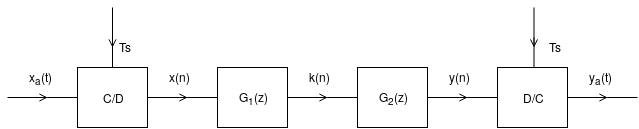
\includegraphics[scale=0.6]{photos/system-diagram.png} \\
    \caption{Given system}
\end{figure}



%------------------------------------------------------------
%   a
\subsection*{a)}
Για το πρώτο μέρος σχετικά με την εύρεση της συνάρτησης μεταφοράς σε Z-Transform γνωρίζουμε ότι ένα LTI system μπορεί να περιγραφεί πλήρως από τη κρουστική απόκριση σε Z-Transform  ή εναλλακτικά μπορούμε να πούμε ως το πηλίκο εξόδου προς εισόδου του, άρα για όλου του συστήματος που ζητείται ισχύει:

% Συνάρτηση μεταφοράς
\begin{align}
    \boxed{H(z)=\frac{Y(z)}{X(z)}} \label{tranf_func}
\end{align}

\par \noindent
Μη γνωρίζοντας άμεσα ούτε το $Y(z)$ ούτε το $X(z)$ πρέπει να βρούμε μέσα από τα δεδομένα ένα τρόπο να τα υπολογίσουμε. Ξέρουμε όμως ότι συνελίξεις στο πεδίο του χρόνου είναι πολλαπλασιασμοί στο πεδίο Ζ οπότε βλέπουμε ότι:

% Συνελίξεις στο χρόνο -> πολλαπλασιασμοί στο Z
\begin{align}
    k(n) = x(n) \circledast g_1(n) \xrightarrow[]{Z} X(z)G_1(z)=K(z) \Rightarrow \boxed{X(z) = \frac{K(z)}{G_1(z)}} \label{first_conv} \\
    y(n) = k(n) \circledast g_2(n) \xrightarrow[]{Z} K(z)G_2(z)=Y(z) \Rightarrow \boxed{Y(z) = K(z)G_2(z)} \label{second_conv}
\end{align}

\par \noindent
Από τις εξισώσεις (\ref{tranf_func}) , (\ref{first_conv}) και (\ref{second_conv}) καταλήγουμε ότι η συνάρτηση μεταφοράς ισούται:

% Από τις παραπάνω που καταλήγουμε για τη συνάρτηση μεταφοράς
\begin{align}
    H(z)&=\frac{K(z)G_2(z)}{\frac{K(z)}{G_1(z)}} \nonumber \\ 
        &=\boxed{G_1(z)G_2(z)} \label{tranf_func_final}
\end{align}

\par \noindent
Το $G_2(z)$ μας δίνεται, οπότε πρέπει να υπολογίσουμε και το $G_1(z)$. Ξέρουμε ότι το $G_1(z)$ περιγράφεται από την εξίσωση διαφορών $k(n) = 0.9k(n-1)+0.2x(n)$ άρα πρώτο βήμα είναι να δημιουργούμε τον Z-Transform του k(n). Για να το κάνουμε αυτό χρησιμοποιούμε την ιδιότητα της μετατόπισης στο χρόνο.
\[ K(z)=0.9z^{-1}K(z)+0.2X(z) \Rightarrow \]

\begin{align}
    \boxed{K(z)=\frac{0.2X(z)}{1-0.9z^{-1}}} \label{k_z_transf}
\end{align}

\par \noindent
Αυτό που παρατηρούμε είναι ότι στην (\ref{k_z_transf}) εμφανίζεται το $X(z)$ συνεπώς από την (\ref{k_z_transf}) και (\ref{first_conv}) καταλήγουμε ότι:

\begin{align}
    \boxed{G_1(z)=\frac{0.2}{1-0.9z^{-1}}} \label{g_1}
\end{align}

\par \noindent
Πλέον έχουμε ότι χρειαζόμαστε για τον υπολογισμό της συνάρτησης μεταφοράς, δηλαδή το $G_1(z)$ και το $G_2(z)$ άρα:

\begin{align}
    H(z)&=G_1(z)G_2(z) \nonumber \\
    &=\frac{0.2}{1-0.9z^{-1}}*\frac{1}{z+0.2} \nonumber \\
    &=\frac{0.2}{(1-0.9z^{-1})(z+0.2)} \nonumber \\
    &=\frac{0.2}{z-0.9+0.2-0.18z^{-1}} \nonumber \\
    &=\frac{0.2}{z-0.7-0.18z^{-1}} \nonumber \\
    &=\boxed{\frac{0.2z^{-1}}{1-0.7z^{-1}-0.18z^{-2}}}
\end{align}

\par \noindent
Όσον αφορά την εξίσωση διαφορών προκύπτει ότι:
\[ H(z)=\frac{Y(z)}{X(z)}=\frac{0.2z^{-1}}{1-0.7z^{-1}-0.18z^{-2}} \Leftrightarrow \]
\[ Y(z) - 0.7z^{-1}Y(z) -0.18z^{-2}Y(z) = 0.2z^{-1}X(z) \]

\par \noindent
Έπειτα υπολογίζουμε τον αντίστροφο μετασχηματισμό Z. %Το σύστημά είναι αιτιατό άρα δεξιόπλευρο συνεπώς ισχύει η ιδιότητα: $\frac{k_i z}{z-a_i} \Leftrightarrow k_i a_i^n u(n)$ άρα:

\[ y(n) - 0.7y(n-1) -0.18y(n-2) = 0.2x(n-1) \Leftrightarrow \]
\begin{align}
    \boxed{y(n) = 0.7y(n-1) + 0.18y(n-2) + 0.2x(n-1)}
\end{align}

%------------------------------------------------------------
%   b
\subsection*{b)}
Αφού είχαμε βρει την συνάρτηση μεταφοράς, μπορούσαμε να σχεδιάσουμε το διάγραμμα πόλων - μηδενικών με την βοήθεια του MATLAB και της συνάρτησης zplane στην οποία θα δίναμε ορίσματα τους συντελεστής των πολυωνύμων του αριθμητή και του παρονομαστή προσέχοντας να είναι συσχετισμένοι οι βαθμοί των πολυωνύμων.

\begin{figure}[H]
    \centering
    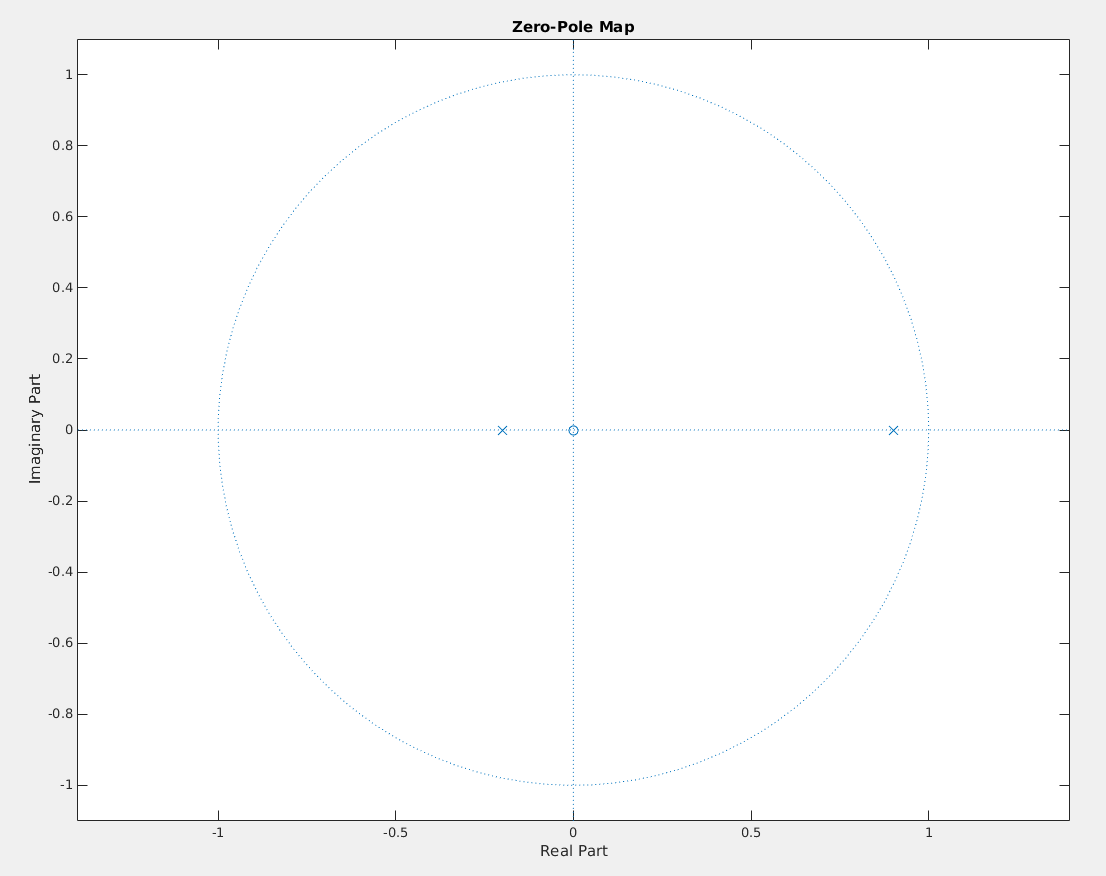
\includegraphics[scale=0.35]{photos/Zero_Pole_Map.png}\\
    \caption{Pole-Zero map on Matlab}
\end{figure}

%------------------------------------------------------------
%   c
\subsection*{c)} 
Για να είναι BIBO ευσταθές το σύστημα, όπως έχουμε δει και από την θεωρία πρέπει να ισχύει ότι ο ROC (Region of convergence) περιλαμβάνει το μοναδιαίο κύκλο $(|z|=1)$. Γενικά ξέρουμε ότι η περιοχή σύγκλισης ορίζεται μόνο από τους πόλους. Επίσης ξέρουμε ότι το σύστημα είναι αιτιατό πράγμα που σημαίνει ότι είναι σίγουρα δεξιόπλευρο. Άρα η περιοχή σύγκλισης του ξεκινάει από ένα κύκλο και εκτείνεται προς το $\pm \infty$ (εξωτερική πλευρά κύκλου με ακτίνα $|r_1|$). 
\par \noindent
Από τα παραπάνω η περιοχή σύγκλισης ικανοποιεί την εξής σχέση $|z|>|r_1|$, με την χρήση του σχεδιαγράμματος μηδενικών - πόλων του β) ερωτήματος βλέπουμε ότι η τιμή του $r_1=0.9$ καθώς γνωρίζουμε ότι δεν μπορεί να περιέχονται πόλοι στη περιοχή σύγκλισης, συνεπώς περιλαμβάνεται ο μοναδιαίος κύκλος σε αυτή, άρα το σύστημα είναι BIBO ευσταθές.

%------------------------------------------------------------
%   d
\subsection*{d)}

%------------------------------------------------------------
%   f
\subsection*{f)}


%---------------------------------------------------------------------------------------------
%   Exercise 2
\section*{Άσκηση 2}
Δίνεται η συνάρτηση μεταφοράς:

$$H(z) = \frac{ 4 - 3.5z^{-1}}{1 - 2.5z^{-1} + z^{-2} } , |z| > 2$$

%------------------------------------------------------------
%   a
\subsection*{a)}
Η θεωρητική ανάλυση της συνάρτησης μεταφοράς είναι η εξής:
\par \noindent
Βρίσκονται οι πόλοι λύνοντας την δευτεροβάθμια εξίσωση.
Σπάει ο αριθμητής και βρίσκονται οι συντελεστές του μέσω της μεθόδου χρήσης των Α-Β.

\[ 1 - 2.5z^{-1} + z^{-2} = 0 \]
\[ Δ = β^2-4αγ = (-2.5)^2-4*1*1 = 6.25 - 4 = 2.25 \]
\[ \sqrt{Δ} = \sqrt{2.25} = 1.5 \]
\[ p_{1,2} = \frac{2.5 \pm \sqrt{Δ}}{2} = \frac{2.5\pm1.5}{2} \Rightarrow p_1=2 \quad \textrm{and} \quad p_2=0.5 \]


\begin{align*}
    \frac{4-3.5z^{-1}}{1-2.5z^{-1}+z^{-2}} &= \frac{A}{1-p_{1}z^{-1}} + \frac{B}{1-p_{2}z^{-1}} \\
    &=\frac{A}{1-2z^{-1}} + \frac{B}{1-0.5z^{-1}} \\
    &=\frac{A(1-0.5z^{-1}) + B(1-2z^{-1})}{(1-2z^{-1})(1-0.5z^{-1})} \Leftrightarrow \\
    & A(1-0.5z^{-1}) + B(1-2z^{-1})=4-3.5z^{-1} \Leftrightarrow \\
    & A - 0.5Az^{-1} + B -2Bz^{-1} = 4 -3.5z^{-1} \Leftrightarrow \\
    & A + B - (0.5A + 2B) = 4 -3.5z^{-1}
\end{align*}

\par \noindent
Συνεπώς:
\[ A+B=4 \Leftrightarrow A=4-B \]
\[ 0.5A+2B=3.5 \Leftrightarrow  A+4B=7 \Leftrightarrow  4-B+4B=7 \Leftrightarrow  3B=3 \Rightarrow  B=1 \quad \textrm{and} \quad  A=3 \]

\par \noindent
Άρα:
$$H(z) =\frac{3}{1-2z^{-1}} + \frac{1}{1-0.5z^{-1}} $$ 

\par \noindent
Το αποτέλεσμα επαληθεύεται μέσω MATLAB:

\begin{figure}[H]
    \centering
   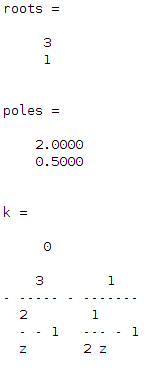
\includegraphics[scale=0.6]{photos/roots_poles_k.png} \\
    \caption{Matlab result}
\end{figure}

%------------------------------------------------------------
%   b
\subsection*{b)}
Το σύστημα είναι αιτιατό για $|z| > 2$.
Για δεξιόπλευρο όρο ισχύει η ιδιότητα:

\[
       \frac{k_i z}{z-a_i} \Leftrightarrow k_i a_i^n u(n)
\] 

\par \noindent
Οπότε προκύπτει το αποτέλεσμα:

\[
    3 * 2^n u(n) + 0.5^n u(n)
\] 

\par \noindent
Το αποτέλεσμα επαληθεύεται μέσω MATLAB:

\begin{figure}[H]
    \centering
    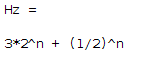
\includegraphics[scale=0.7]{photos/H_z.png} \\
    \caption{Matlab result }
\end{figure}

\end{document}